\documentclass[
  parskip=half,
  bibliography=totoc,     % Literatur im Inhaltsverzeichnis
  captions=tableheading,  % Tabellenüberschriften
  titlepage=firstiscover, % Titelseite ist Deckblatt
]{scrartcl}

% LaTeX2e korrigieren.
\usepackage{fixltx2e}
% Warnung, falls nochmal kompiliert werden muss
\usepackage[aux]{rerunfilecheck}

% deutsche Spracheinstellungen
\usepackage{polyglossia}
\setmainlanguage{german}

% unverzichtbare Mathe-Befehle
\usepackage{amsmath}
% viele Mathe-Symbole
\usepackage{amssymb}
% Erweiterungen für amsmath
\usepackage{mathtools}

% Fonteinstellungen
\usepackage{fontspec}
\defaultfontfeatures{Ligatures=TeX}

\usepackage[
  math-style=ISO,    % \
  bold-style=ISO,    % |
  sans-style=italic, % | ISO-Standard folgen
  nabla=upright,     % |
  partial=upright,   % /
]{unicode-math}

\setmathfont{Latin Modern Math}
\setmathfont[range={\mathscr, \mathbfscr}]{XITS Math}
\setmathfont[range=\coloneq]{XITS Math}
\setmathfont[range=\propto]{XITS Math}
% make bar horizontal, use \hslash for slashed h
\let\hbar\relax
\DeclareMathSymbol{\hbar}{\mathord}{AMSb}{"7E}
\DeclareMathSymbol{ℏ}{\mathord}{AMSb}{"7E}

% richtige Anführungszeichen
\usepackage[autostyle]{csquotes}

% Zahlen und Einheiten
\usepackage[
  locale=DE,                   % deutsche Einstellungen
  separate-uncertainty=true,   % Immer Fehler mit \pm
  per-mode=symbol-or-fraction, % m/s im Text, sonst Brüche
]{siunitx}

% chemische Formeln
\usepackage[version=3]{mhchem}

% schöne Brüche im Text
\usepackage{xfrac}

% Floats innerhalb einer Section halten
\usepackage[section, below]{placeins}
% Captions schöner machen.
\usepackage[
  labelfont=bf,        % Tabelle x: Abbildung y: ist jetzt fett
  font=small,          % Schrift etwas kleiner als Dokument
  width=0.9\textwidth, % maximale Breite einer Caption schmaler
]{caption}
% subfigure, subtable, subref
\usepackage{subcaption}

% Grafiken können eingebunden werden
\usepackage{graphicx}
% größere Variation von Dateinamen möglich
\usepackage{grffile}

% Standardplatzierung für Floats einstellen
\usepackage{float}
\floatplacement{figure}{htbp}
\floatplacement{table}{htbp}

% schöne Tabellen
\usepackage{booktabs}

% Seite drehen für breite Tabellen
\usepackage{pdflscape}

% Literaturverzeichnis
\usepackage{biblatex}
% Quellendatenbank
\addbibresource{lit.bib}
\addbibresource{programme.bib}

% Hyperlinks im Dokument
\usepackage[
  unicode,
  pdfusetitle,    % Titel, Autoren und Datum als PDF-Attribute
  pdfcreator={},  % PDF-Attribute säubern
  pdfproducer={}, % "
]{hyperref}
% erweiterte Bookmarks im PDF
\usepackage{bookmark}

% Trennung von Wörtern mit Strichen
\usepackage[shortcuts]{extdash}

\title{V203: Verdampfungswärme und Dampfdruckkurve}
\author{
  Simon Schulte \\
  \texorpdfstring{
    \href{mailto:simon.schulte@udo.edu}{simon.schulte@udo.edu}\and}{, }
  Tim Sedlaczek \\
  \texorpdfstring{
    \href{mailto:tim.sedlaczek@udo.edu}{tim.sedlaczek@udo.edu}}{}
}
\date{Durchführung: 29.11.2016\\
      Abgabe: 6.12.2016}
\begin{document}
\newpage
\maketitle
\tableofcontents
\newpage

\section{Zielsetzung}
\label{sec:zielsetzung}
In dem Versuch soll die Dampfdruckkurve von Wasser aufgenommen werden. Daraus
wird dann die Verdampfungswärme $L$ errechnet. Außerdem wird die
Temperaturabhängigkeit der Verdampfungswärme bestimmt.
\section{Theorie}
\label{sec:theorie}
Die drei Aggregatzustände von Wasser sind nicht absolut fest. So ist es bei
\SI{0}{\celsius} möglich, dass Wasser alle drei Aggregatzustände annimmt, also
sowohl fest, flüssig als auch gasförmig ist. Wenn man nun die Temperatur von
Wasser ändert und ein Inertialsystem erzeugt, in welchem man den Druck variieren
kann, ändert sich das Zustandsdiagramm von Wasser. In der Abbildung 1 zu sehen
ist das qualitative Zustandsdiagramm von Wasser.
\begin{figure}[htb]
  \centering
  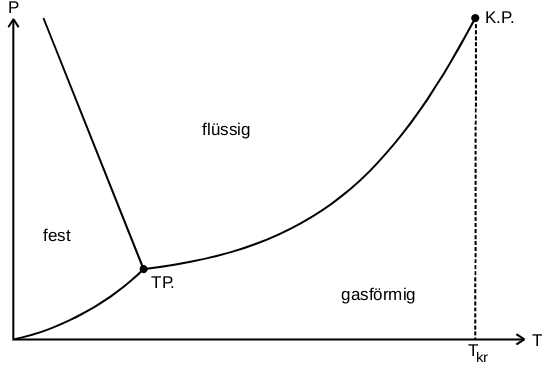
\includegraphics[width=0.8\textwidth]{Aggregatzustände.png}
  \caption{Qualitatives Zustandsdiagramm von Wasser}
  \label{fig:aggregatzustände}
\end{figure}
Die Kurve von dem Punkt TP. zu K.P. nennt sich Dampfdruckkurve. Auf dieser
existieren zwei Aggregatzustände gleichzeitig, in diesem Fall flüssig und
gasförmig. Der Verlauf dieser Kurve wird durch die Verdampfungswärme $L$
festgelegt.
Um die Dampfdruckkurve eines Stoffes zu berechnen, nutzt man die
Clausius-Clapeyronsche Gleichung
\begin{equation}
  (V_D-V_F)\,\symup{d}\,\rho=\,\frac{L}{T}\,\symup{d}\,T
\end{equation}
\label{eq:formel1}
$V_D$, $V_F$ und $L$ sind Funktionen der Temperatur. $T$ ist die Temperatur
selbst und $\rho$ ist der Druck. Da bei der Integration der Clausius-Clapeyronschen
Gleichung $V_D$, $V_F$ und $L$ mitunter sehr kompliziert werden können, nähert
man diese folgendermaßen:
$V_F$ ist gegenüber $V_D$ vernachlässigbar, $V_D$ gehorcht der idealen
Gasgleichung
\begin{equation}
  V_D\,(\rho,\,T)\,=\,R\,\frac{T}{\rho}
\end{equation}
\label{eq:formel2}
und $L$ ist druck- und temperaturunabhängig. Dadurch ergibt sich für Gleichung
(1)
\begin{equation}
  \frac{R}{\rho}\,\symup{d}\rho\,=\,\frac{L}{T²}\,\symup{d}T
\end{equation}
\label{eq:formel3}
Wenn man dies nun integriert ergibt sich
\begin{equation}
  ln\rho\,=\,-\,\frac{L}{R}\,\cdot\frac{1}{T}\,+\,const
\end{equation}
\label{eq:formel4}
wobei $\rho$ der Druck ist, $R$ die allgemeine Gaskonstante und $L$
die Verdampfungswärme.
Die Allgemeine Gasgleichung ist gegeben durch
\begin{equation}
  \rho\,\cdot\,V\,=\,n\,\cdot\,R\,\cdot\,T
\end{equation}
\label{eq:formel6}
\newpage
\section{Durchführung}
\label{sec:durchführung}
\subsection{Versuchsaufbau}
\label{sec:versuchsaufbau}

Die Apparatur für die Messungen im Druckbereich $\rho$ $\le$ \SI{1}{\bar} ist
wie in Abbildung 2 aufgebaut.
Ein elektrisch beheizbarer Mehrhalskolben, gefüllt mit etwas Wasser, ist über
einen Rückflusskühler und eine Woulfsche Flasche mit einem Barometer und einer
Wasserstrahlpumpe verbunden. Der Rückflusskühler schützt das Barometer vor
Feuchtigkeit, indem aufsteigender Wasserdampf an ihm kondesieren kann. Die
Woulfsche Flasche schützt die Apparatur vor versehentlichem Eindringen kalten
Wassers durch die Wasserstrahlpumpe.
\begin{figure}[htb]
  \centering
  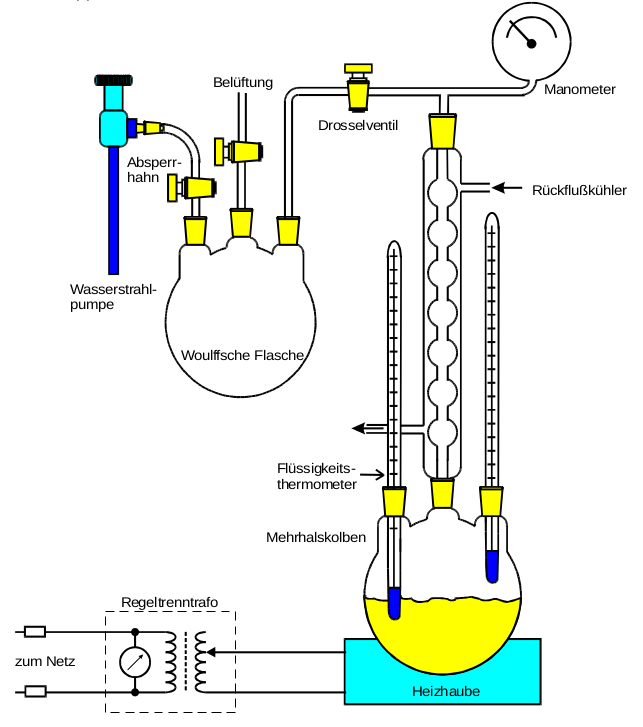
\includegraphics[width=0.8\textwidth]{Versuch1.png}
  \caption{Skizze der für den Druckbereich $\rho$\,$<$\,\SI{1}{\bar} verwendeten Messapparatur}
  \label{fig:versuch1}
\end{figure}
Die Apparatur für die Messungen im Druckbereich \num{1}\,$<$\,$\rho$\,$<$\,\SI{15}{\bar}
ist wie in Abbildung 3 aufgebaut.
Die Wasserprobe befindet sich hierbei in einem Stahlzylinder, der, ebenfalls
elektrisch beheizt, weitaus höheren Drücken standhält. Dieser ist über ein
U-Rohr mit einem Drucksensor verbunden, welcher durch eine kleine Kühlschale mit
Wasser vor dem Überhitzen geschützt wird. Wie im ersten Aufbau ist auch hier ein
Thermometer in direkter Nähe zur Probe angebracht, wobei allerdings nun mit
einem digitalen Thermometer gearbeitet wird.
\begin{figure}[htb]
  \centering
  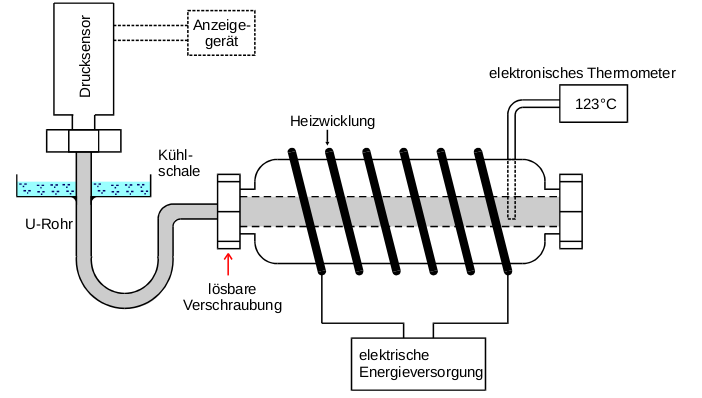
\includegraphics[width=0.8\textwidth]{Versuch2.png}
  \caption{Skizze der für den Druckbereich \num{1}\,$<$\,$\rho$\,$<$\,\SI{15}{\bar} verwendeten Messapparatur}
  \label{fig:versuch2}
\end{figure}
\subsection{Versuchsdurchführung}
\label{sec:versuchsdurcführung}
Das Experiment besteht aus zwei Teilversuchen. Im ersten Versuch wird die
Dampfdruckkurve von Wasser im Druckbereich zwischen \num{85} und
\SI{1000}{\milli\bar} ermittelt. Zunächst wird mithilfe der Wasserstrahlpumpe
die Glasapparatur evakuiert und der Innendruck somit soweit wie möglich gesenkt.
Danach werden alle Ventile geschlossen, der Rückflusskühler und die Heizhaube
werden eingeschaltet. Über das Thermometer, welches sich in der Dampfphase
oberhalb des Wassers befindet und das Barometer lassen sich, bei eingeschalteter
Heizhaube, laufend Wertepaare von Temperatur und Druck aufnehmen. Dabei wird in
\SI{5}{\milli\bar} Schritten zwischen \num{85} und \SI{200}{\milli\bar}
gemessen und in \SI{50}{\milli\bar} Schritten zwischen \num{200} und
\SI{1000}{\milli\bar} gemessen.
Wie im ersten Versuchsabschnitt wird die Probe nun kontinuierlich erhitzt, wobei
Temperatur- und Druckverlauf protokolliert werden. Gemessen wird im Druckbereich
zwischen \num{1} und \SI{15}{\bar}.
\section{Auswertung}
\label{sec:auswertung}
Die in der Auswertung verwendeten Mittelwerte mehrfach gemessener Größen sind
gemäß der Gleichung
\begin{equation}
    \bar{x}=\frac{1}{n}\sum_{i=1}^n x_i
\end{equation}
\label{eq:formel7}
bestimmt. Die Standardabweichung des Mittelwertes ergibt sich dabei zu
\begin{equation}
    \mathup{\Delta}\bar{x}=\sqrt{\frac{1}{n(n-1)}\sum_{i=1}^n\left(x_i-\bar{x}\right)^2}.
\end{equation}
\label{eq:formel8}
Resultiert eine Größe über eine Gleichung aus zwei anderen fehlerbehafteten
Größen, so berechnet sich der Gesamtfehler nach der Gaußschen
Fehlerfortpflanzung zu
\begin{equation}
    \mathup{\Delta}f(x_1,x_2,...,x_n)=\sqrt{\left(\frac{\mathup{d}f}{\mathup{d}x_1}\mathup{\Delta}x_1\right)^2+\left(\frac{\mathup{d}f}{\mathup{d}x_2}\mathup{\Delta}x_2\right)^2+ \dotsb +\left(\frac{\mathup{d}f}{\mathup{d}x_n}\mathup{\Delta}x_n\right)^2}.
\end{equation}
\label{eq:formel9}
\section{Literatur}
[1]Besucht am 2.12.2016, Die allgemeine Gasgleichung,
URL:http://grund-wissen.de/physik/waermelehre/allgemeine-gasgleichung.html
[2]TU Dortmund. Verdampfungswärme und Dampfdruck-Kurve, besucht am 2.12.2016
URL:http://129.217.224.2/HOMEPAGE/PHYSIKER/BACHELOR/AP/SKRIPT/V203.pdf
\end{document}
